\begin{abstract}
We consider a matched subspace detection problem where the signal is placed deterministically in an unknown location in an unknown subspace which is estimated from noisy signal-bearing training data with missing entries. This subspace estimate is inaccurate due to both limited training data and missing entries in the training data matrix. Recent results from random matrix theory precisely quantify these subspace estimation errors. We derive an optimal detector which accounts for these  subspace estimation errors and use an ROC analysis to show that the optimal MSD outperforms the typical plug-in detector which assumes that the subspace estimate is exact. This increase in performance arises from the optimal detector only using the $k_\text{eff}\leq k$ informative signal subspace components. The percent of missing data helps determine $k_\text{eff}$. Detection better than random guessing is only achievable when the percent of missing data is below a critical threshold.
\end{abstract}
%
\begin{keywords}
Mathced subspace detector, random matrix theory, missing data, ROC analysis
\end{keywords}
%
\section{Introduction}\label{sec:intro}

The matched subspace detector (MSD) is a widely used tool in signal processing and machine learning to detect a signal embedded in a low-rank subspace in the presence of additive noise \cite{scharf1994matched,jin2005cfar,mcwhorter2003matched}. The performance of the MSD has been explored when the low-rank signal subspace is known. Scharf and Friedlander \cite{scharf1994matched} consider the MSD when the signal is placed deterministically at an unknown location in a known subspace while McWhorter and Scharf \cite{mcwhorter2003matched} extend this work to allow the signal to be placed randomly in the known subspace.

Limited work is available, however, when the signal subspace is unknown or when the training data has missing entries. Asendorf and Nadakuditi \cite{asendorf2011msd} characterize the performance of the stochastic MSD with an unknown signal subspace. They used random matrix theory (RMT) to show the importance of using $k_\text{eff}\leq k$ informative signal subspace components in detector statistics. RMT precisely quantifies errors in subspace estimation arising from limited training data and missing data. This paper will characterize the performance of the MSD which accounts for these subspace estimation errors in the setting when the signal is placed deterministically in the unknown low-rank subspace and the training data contains missing entries.

An ROC analysis shows the importance of selecting $k_\text{eff}\leq k$ informative signal subspace components as in \cite{asendorf2011msd}. The percentage of missing entries in the training data plays a vital role in the performance of the MSD. When too many entries are missing, detection performance deteriorates to random guessing.

The paper is organized as follows. Section \ref{sec:prob stat} formally states the detection problem. Section \ref{sec:rmt} presents pertinent results from RMT. These results are used in Section \ref{sec:derive} to derive a plug-in and optimal MSD and in Section \ref{sec:roc} to derive theoretical ROC curves for each detector. Section \ref{sec:results} validates our analytical predictions, highlights the importance of selecting $k_\text{eff}$ over $k$ subspace components, and demonstrates the effect of missing data. Concluding remarks are provided in Section \ref{sec:conclusion}.

\section{Problem Statement}\label{sec:prob stat}

We consider the detection problem where our observation vector $y \in \mathbb{C}^{n \times 1}$ is modeled as follows:
\begin{equation}
y=\left\{
\begin{aligned}
&z
&& y\in H_0\\
&U\Sigma x+z
&& y\in H_1\\
\end{aligned}\right.
\end{equation}
where $z\sim\mathcal{N}(0,I_n)$, $U$ is an unknown $n\times k$ (real or complex) matrix with orthonormal columns, $\Sigma=\diag(\sigma_1,\dots,\sigma_k)$ is known with $\sigma_1>\sigma_2>\dots>\sigma_k>0$, and $x\in\mathbb{C}^{k\times 1}$ is an unknown deterministic vector. The dimension of our subspace, $k$, is known and $k\ll n$. We also assume that $x$ and $z$ are independent.

To estimate our unknown subspace, $U$, we are given independent signal-bearing training data $\{y_1,\dots,y_m\}$, with $y_i\in H_1 \text{ for } i=1,\dots,m$. Each $y_i$ is assumed to be generated from a unique $x$. However, only a portion of our training data, $0\leq p\leq 1$, is actually observed. $p$ is known and represents the equal probability, $p$, that an entry in the training data matrix is present. Missing entries in our training data matrix are represented with zeros. After forming our subspace estimate, $\widehat{U}$,  we generate a $k \times 1$ test vector $w=\widehat{U}^Hy$. Our goal is to determine a detector, $g(w)\to\{H_0,H_1\}$ which solves the following problem for an unlabeled testing point, $w$:
\begin{equation}\label{eq:maximization}
\begin{aligned}
&\text{maximize}
&& P_D=P\left(g(w)\to H_1 | w\in H_1\right)\\
&\text{subject to}
&& P_F=P\left(g(w)\to H_1 | w\in H_0\right)\leq\alpha\\
\end{aligned}
\end{equation}
where $\alpha\in[0,1]$.

\section{Pertinent Results from RMT}\label{sec:rmt}

The first step in any detector derivation is to form an estimate $\widehat{U}$ to use in a GLRT. We are given signal-bearing training data $\{y_1,\dots,y_m\}$ where $y_i\in H_1$, for $i=1,\dots,m$. which are stacked as columns in a matrix $Y=[y_1,\dots,y_m]$. Recall that our training data contains missing entries such that we only have a fraction $p$ of the entries of $Y$. To form an estimate of $U$, we take the $k$ leftmost left singular vectors from the SVD of $Y$. Recent results from random matrix theory allow us to classify the accuracy of the singular vectors of $Y$. From \cite{benaych2011singular} we have the following result.

\begin{Th}\label{th:angles}
As $n,m \longrightarrow \infty$ with $n/m \to c$ we have that:
\begin{equation*}
\begin{aligned}
&|\langle u_i,\widehat{u}_i\rangle|^2\convas
\begin{cases}
1-\dfrac{c\left(1+p\sigma_i^2\right)}{p\sigma_i^2\left(p\sigma_i^2 + c\right)} & \text{ if } \sigma_{i}>\frac{c^{1/4}}{\sqrt{p}}\\
0 & \textrm{otherwise}\\
\end{cases}\\
&|\langle u_i,\widehat{u}_j\rangle|^2\convas 0 \qquad \textrm{ for } i \neq j\\
\end{aligned},
\end{equation*}
where $\widehat{u}_i$ is the $i^{\text{th}}$ left singular vector of $Y$ where $i,j=1,\dots,n$.
\end{Th}

Note that the proof of the case where $i\neq j$ will appear in a later journal publication \cite{asendorf}. The key point of Theorem \ref{th:angles} is that only the singular vectors corresponding to signal singular values above the phase transition $\frac{c^{1/4}}{\sqrt{p}}$ are \textit{informative}. When a signal singular value drops below this critical threshold, the corresponding singular vector estimate is essentially noise-like  (i.e. $|\langle u_i,\widehat{u}_i\rangle|^2=o_{p}(1)$) and thus \textit{uninformative}. The term $|\langle u_i,\widehat{u}_i\rangle|^2$ quantifies mismatch between the estimated and underlying singular vectors and plays an important role in the performance analysis of the resulting detectors. Intuitively we expect a degradation in the performance of detectors  that utilize subspace components for which $|\langle u_i,\widehat{u}_i\rangle|^2=o_{p}(1)$.  We refer to the estimate in Theorem \ref{th:angles} as $|\langle u_i,\widehat{u}_i\rangle|^2_{\text{rmt}}$.

\section{Family of Matched Subspace Detectors}\label{sec:derive}

The Neyman-Pearson Lemma (see \cite{van1968detection}) states that the solution to (\ref{eq:maximization}) is a likelihood ratio test (LRT)
\begin{equation*}
\Lambda(w) \detgtrless \eta
\end{equation*}
where $\Lambda(w) = \frac{f(w|H_1)}{f(w|H_0)}$ and $\eta$ satisfies $P(\Lambda(w)\leq\eta|H_0)=\alpha$. The LRT relies on the conditional distributions of our test statistic under each hypothesis, which by properties of Gaussian random variables are simply
\begin{equation*}
\begin{aligned}
&w|H_0\sim\mathcal{N}(0,I_{k})\\
&w|H_1\sim\mathcal{N}(\widehat{U}^HU\Sigma x, I_{k}).\\
\end{aligned}
\end{equation*}
However, as $x$ is unknown, we employ the generalized likelihood ration test (GLRT) where $\Lambda(w) = \frac{\max_x f(w|H_1)}{f(w|H_0)}$. The GLRT statistic for our processed data $w$ is
\begin{equation*}
\Lambda(w)=\frac{\max_x\mathcal{N}(\widehat{U}^HU\Sigma x,I_{k})}{\mathcal{N}(0,I_{k})}.
\end{equation*}
Employing maximum likelihood estimation on $x$ yields the estimate $\widehat{x}=\left(\Sigma U^H\widehat{U}\widehat{U}^HU\Sigma\right)^{-1}\Sigma U^H\widehat{U}w$. After simplification of the GLRT using $\widehat{x}$ and using the natural logarithm operator as a monotonic operation, the GLRT statistic becomes
\begin{equation}\label{eq:oracle stat}
\Lambda(w) = w^H\left(\widehat{U}^HU\Sigma\left(\Sigma U^H\widehat{U}\widehat{U}^HU\Sigma\right)^{-1}\Sigma U^H\widehat{U}\right)w
\end{equation}
and the detector is
\begin{equation}\label{eq:oracle classifier}
\Lambda(w) \detgtrless 2\ln(\eta)
\end{equation}
where $\eta$ satisfies $P(\Lambda(w)\leq2\ln\left(\eta\right)|H_0)=\alpha$.

%\begin{table*}[!ht]
%\centering
%\begin{tabular}{cclclcl}\toprule
% Detector & \phantom{a} & Detector Statistic $\Lambda(w)$ & \phantom{a} & Null Hypothesis Distribution $\Lambda|H_0$& \phantom{a} & Simple Hypothesis Distribution $\Lambda|H_1$\\
%\midrule
%Plug-in && $\sum_{i=1}^{k}w_i^2$ && $\chi_k^2$ && $\chi_{\text{nc}}^2(k,\delta)$\\
% Optimal&& $\sum_{i=1}^{k_\text{eff}}w_i^2$ && $\chi_{k_\text{eff}}^2$ && $\chi_\text{nc}^2(k_\text{eff},\delta)$\\
%\bottomrule
%\end{tabular}
%\caption{Given an observation vector $y$ we form the vector $w=\widehat{U}^Hy$ where $\widehat{U}$ is an estimate of the signal subspace. The table summarizes the test statistic associated with each detector and the associated distribution under $H_0$ and $H_1$. Here $\delta=\sum_{i=1}^{k_\text{eff}}\sigma_i^2|\langle u_s,\widehat{u}_i\rangle|^2x_i^2$. In the CFAR setting, the threshold is  set to obtain the desired false alarm probability. Note the appearance of $k_\text{eff}$ in the optimal detector.}\vskip-0.2cm
%\label{table: main results}
%\end{table*}

\subsection{Plug-in Detector}

In our problem statement, $U$ is unknown, and therefore (\ref{eq:oracle stat}) cannot be computed directly. One may then substitute a ML estimate for $U$ in (\ref{eq:oracle stat}) as in \cite{jin2005cfar} and \cite{mcwhorter2003matched}. The ML estimate (in the large-sample, small matrix setting) for $U$ is:
\begin{equation}\label{eq:param estims}
\begin{aligned}
&\widehat{U}=[\widehat{u}_1 \dots \widehat{u}_{k}]\\
\end{aligned}
\end{equation}
where $\widehat{u}_1,\dots,\widehat{u}_{k}$ are the left singular vectors corresponding to the largest $k$ singular values of $Y$.

By replacing the unknown parameters in (\ref{eq:oracle stat}) with the estimated parameters in (\ref{eq:param estims}), the plug-in detector statistic becomes
\begin{equation*}
\Lambda_{\text{plugin}}(w)= w^H\left(\widehat{U}^H\widehat{U}\Sigma\left(\Sigma\widehat{U}^H\widehat{U}\widehat{U}^H\widehat{U}\Sigma\right)^{-1}\Sigma\widehat{U}^H\widehat{U}\right)w.\\
\end{equation*}
This simplifies to
\begin{equation}\label{eq:plugin stat}
\boxed{\Lambda_{\text{plugin}}(w) = w^Hw=\sum_{i=1}^kw_i^2}
\end{equation}
and our detector becomes
\begin{equation}\label{eq:plugin classifier}
\boxed{\Lambda_{\text{plugin}}(w) \detgtrless 2\ln(\eta_{\text{plugin}})}
\end{equation}
where $\eta_{\text{plugin}}$ satisfies $P(\Lambda_{\text{plugin}}(w)\leq2\ln\left(\eta_{\text{plugin}}\right)|H_0)=\alpha$.

The plug-in detector assumes that the estimated signal subspace $\widehat{U}$ is equal to the true signal subspace $U$. However, as shown in Section \ref{sec:rmt}, using uniformative components of $w$ is not well motivated.

\subsection{Optimal Detector}\label{subsec:optdet}

Consider the the term $\widehat{U}^HU$. By Theorem \ref{th:angles} and additional analysis omitted here for brevity (see \cite{asendorf}), we have that in the large matrix limit $\widehat{U}^HU=SA$ where $S=\diag(s_1,\dots,s_{k})$ with $s_i=\pm1$ (random phase) and $A=\diag(a_1,\dots,a_k)$ with $a_i=|\langle u_i,\widehat{u}_i\rangle|$.

The plug-in detector assumes that $A=S=I_k$, that is $s_i=1$ and $|\langle u_i,\widehat{u}_i\rangle|=1$ . However, as seen in Section \ref{sec:rmt}, this assumption is invalid. Let us now re-derive the GLRT using Theorem \ref{th:angles}. Our conditional distributions are
\begin{equation*}
\begin{aligned}
&w|H_0\sim\mathcal{N}(0,I_{k})\\
&w|H_1\sim\mathcal{N}(SA\Sigma x, I_{k})\\
\end{aligned}
\end{equation*}
and the GLRT is
\begin{equation*}
\Lambda(w)=\frac{\max_x\mathcal{N}(SA\Sigma x,I_{k})}{\mathcal{N}(0,I_{k})}.
\end{equation*}
Since the covariance matrices are diagonal and $S$, $A$, and $\Sigma$ are diagonal, we have that
\begin{equation*}
\max_x\mathcal{N}(SA\Sigma x,I_{k})=\prod_{i=1}^k\max_{x_i}\mathcal{N}(\sigma_is_ia_ix_i,1).
\end{equation*}
We use Theorem \ref{th:angles} to estimate $a_i=\sqrt{|\langle u_i,\widehat{u}_i\rangle|^2_{\text{rmt}}}$. Now, $a_i=0$ when $\sigma_i\leq \frac{c^{1/4}}{\sqrt{p}}$. We define $k_\text{eff}$ as the number of signal singular values above the phase transition $\frac{c^{1/4}}{\sqrt{p}}$. Our GLRT becomes
\begin{equation*}
\Lambda(w)=\frac{\mathcal{N}(0,1)^{k-k_\text{keff}}\prod_{i=1}^{k_\text{eff}}\max_{x_i}\mathcal{N}(\sigma_is_ia_ix_i,1)}{\mathcal{N}(0,I_{k})}.
\end{equation*}
Employing maximum likelihood estimation on the remaining $x_i$ yields the estimates $\widehat{x}_i=\frac{w_i}{s_ia_i}$. Notice that for these values of $x_i$, dividing by $a_i$ is justified as the corresponding signal singular value is above the phase transition and so $a_i>0$. After simplification of the GLRT using this $\widehat{x}_i$ and the natural logarithm operator, the statistic becomes
\begin{equation}\label{eq:opt stat}
\boxed{\Lambda_{\text{rmt}}(w) = \sum_{i=1}^{k_\text{eff}}w_i^2}
\end{equation}
and our detector becomes
\begin{equation}\label{eq:opt classifier}
\boxed{\Lambda_{\text{rmt}}(w) \detgtrless 2\ln(\eta_{\text{rmt}})}
\end{equation}
where $\eta_{\text{rmt}}$ satisfies $P(\Lambda_{\text{rmt}}(w)\leq2\ln\left(\eta_{\text{rmt}}\right)|H_0)=\alpha$.

\section{Theoretical ROC Curve Derivation}\label{sec:roc}
A standard way to compare the plug-in and optimal detectors derived in (\ref{eq:plugin classifier}) and (\ref{eq:opt classifier}) respectively is to compute their ROC curves \cite{fawcett2006introduction}. For a particular statistic $\Lambda(w)$, to compute theoretical ROC curves, we must compute
\begin{equation}\label{eq:target cdf}
\begin{aligned}
&P_D = P(\Lambda(w) \geq \gamma| w\in H_1)\\
&P_F = P(\Lambda(w) \geq \gamma| w\in H_0)\\
\end{aligned}
\end{equation}
for $-\infty<\gamma<\infty$. To do this, we explore the conditional CDF under each hypothesis for the statistics (\ref{eq:plugin stat}) and (\ref{eq:opt stat}).

The conditional distribution of a test sample under $H_0$ is $w|H_0\sim\mathcal{N}(0,I_k)$. Clearly $\Lambda_\text{plugin}(w)|H_0\sim\chi_k^2$ and $\Lambda_\text{rmt}(w)\sim\chi_\text{eff}^2$. The conditional distribution under $H_1$ is $w|H_1\sim\mathcal{N}(\widehat{U}^HU\Sigma x,I_k)$. As argued in Section \ref{subsec:optdet}, $\widehat{U}^HU=SA$ is asymptotically diagonal. We have that $w_i|H_1\approx\mathcal{N}(a_is_i\sigma_ix_i,1)$ are i.i.d for $i=1,\dots,k$. Therefore $\Lambda_\text{plugin}(w)|H_1\sim\chi_\text{nc}^2(k,\delta)$ and $\Lambda_\text{rmt}(w)|H_1\sim\chi_\text{nc}^2(k_\text{eff},\delta)$ where
\begin{equation}\label{eq:delta}
\delta=\sum_{i=1}^k\sigma_i^2|\langle u_s,\widehat{u}_i\rangle|^2x_i^2=\sum_{i=1}^{k_\text{eff}}\sigma_i^2|\langle u_s,\widehat{u}_i\rangle|^2x_i^2
 \end{equation}
is the noncentrality parameter for the noncentral chi-square distribution with $k$ degrees of freedom. An analytical expression for the asymptotic performance in the large matrix limit  is obtained by substituting expressions from Theorem \ref{th:angles} in (\ref{eq:delta}). To compute a theoretical ROC curve, we may solve for $\gamma$ in terms of $P_F$ and substitute this into the expression for $P_D$. Doing so yields
\begin{equation}\label{eq:roc}
\begin{aligned}
&P_{D_\text{plugin}}=1-Q_{\chi_\text{nc}^2(k,\delta)}\left(Q^{-1}_{\chi^2_k}\left(1-P_F\right)\right)\\
&P_{D_\text{rmt}}=1-Q_{\chi_\text{nc}^2(k_\text{eff},\delta)}\left(Q^{-1}_{\chi^2_{k_\text{eff}}}\left(1-P_F\right)\right)
\end{aligned}
\end{equation}
where $Q$ is the appropriate cdf. Figure \ref{fig:roc1} illustrates the result of one such computation.

\section{Simulation Results and Discussion}\label{sec:results}

\begin{figure}
\centering
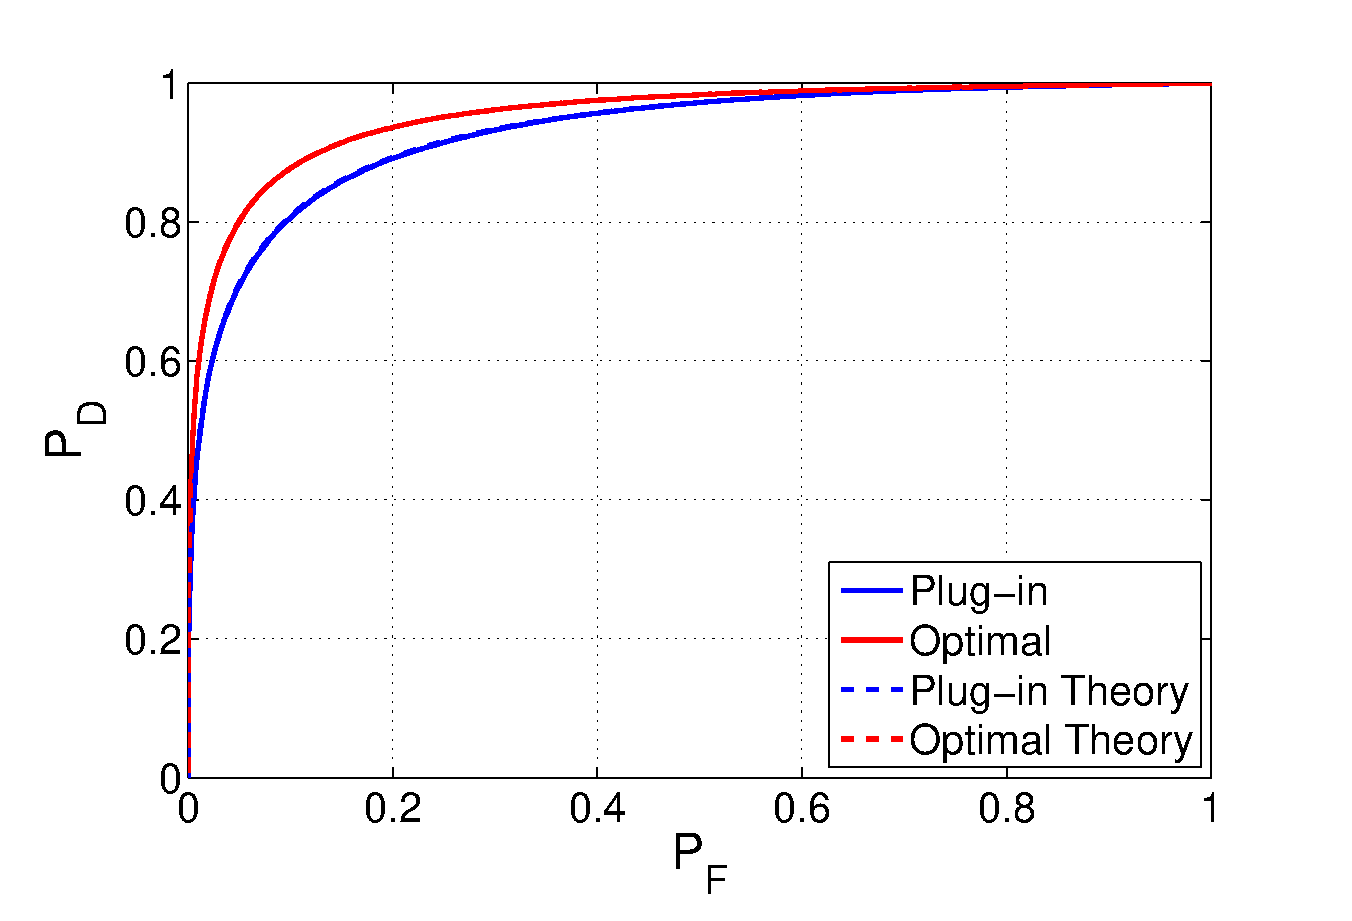
\includegraphics[width=3.5in]{figures/basic_roc.eps}
\caption{Empirical and theoretical ROC curves for the plug-in and optimal matched subspace detectors. Empirical ROC curves were simulated with $n=500$, $m=500$, $k=2$, $\Sigma=\diag(3,0.1)$, and $p=0.8$. However, as $\sigma_2$ is below the critical threshold, $k_{\text{eff}} = 1$. The empirical ROC curves were computed using $5000$ test samples and averaged over 25 trials using algorithms 2 and 4 of \cite{fawcett2006introduction}. $x$ was generated randomly but was the same for every trial. The theoretical ROC curves were computed by \ref{eq:roc}. The theoretically predicted ROC curves match the empirical results reflecting the accuracy of the approximations employed. We observe a performance gain when using the optimal detector.}\vskip-0.15cm
\label{fig:roc1}
\end{figure}

\begin{figure}
\centering
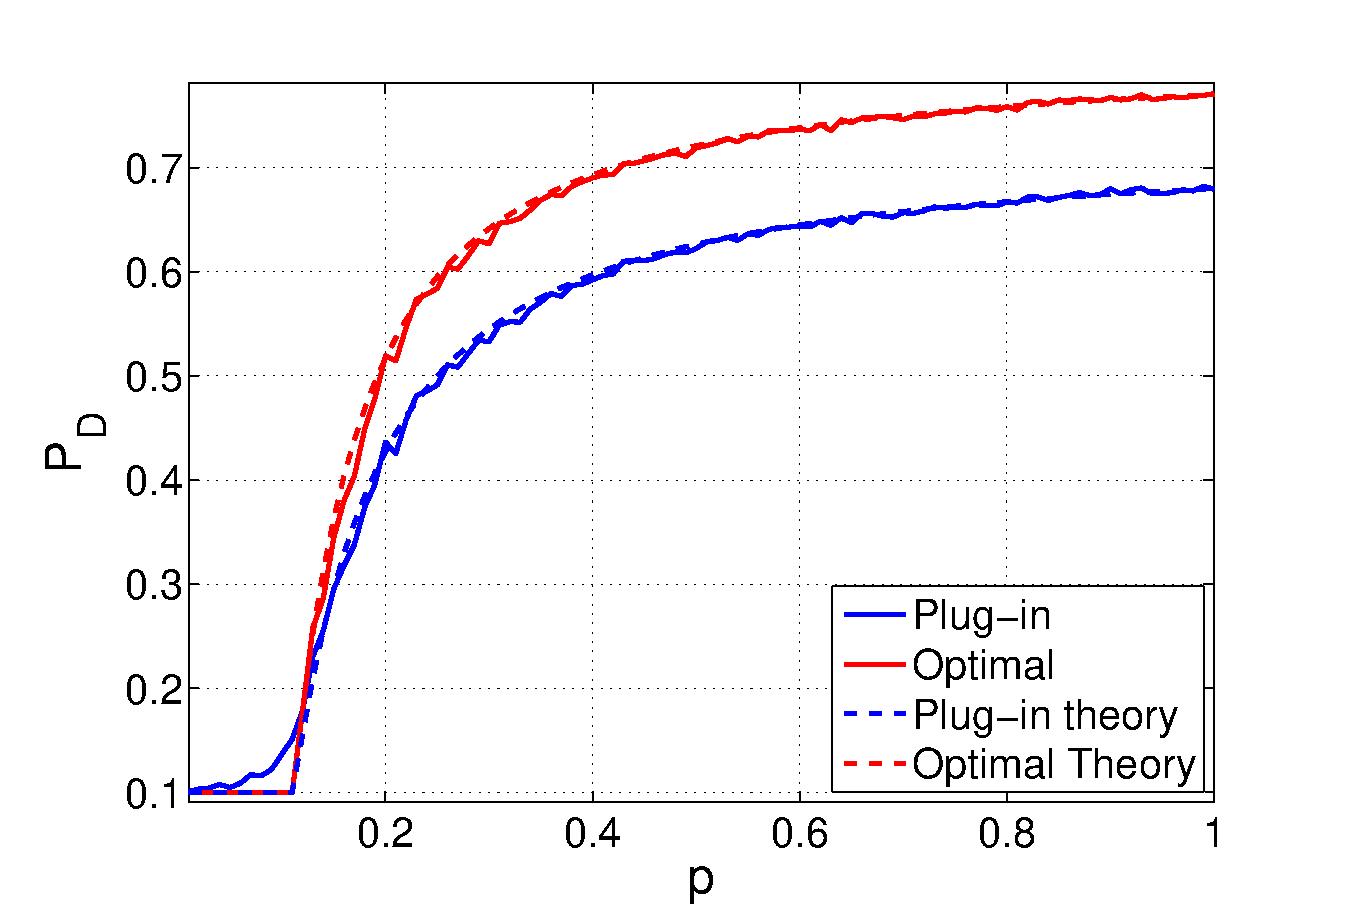
\includegraphics[width=3.5in]{figures/sparsity.eps}
\caption{Empirical exploration of the achieved probability of detection, $P_D$, for a fixed probability of false alarm, $P_F=0.1$, for various $p$. For the simulation, $n=1000$, $m=1000$, $k=2$, $\Sigma=\diag(3,0.1)$. $P_D$ calculation was computed using 5000 test samples and averaged over 25 trials. $x$ was generated randomly but was the same for every trial and value of $p$. For low values of $p$, $k_\text{eff}=0$ and performance degrades to $P_D=P_F$ for both detectors. As $p$ increases, $k_\text{eff}=1$ allowing the detectors to achieve better than random guessing performance. When $k_\text{eff}>0$ the plug-in detector is sub-optimal for all values of $p$.}\vskip-0.15cm
\label{fig:sparsity}
\end{figure}

\subsection{ROC Curves}

As seen in Figure \ref{fig:roc1}, for any false alarm rate ($P_F$), the optimal detector achieves a higher probability of detection ($P_D$, demonstrating the sub-optimality of the plug-in detector. This is expected because $k_\text{eff}<k$ so that there are uniformative subspace components. The theoretical ROC curves in (\ref{eq:roc}) match the empirically generated ROC curves validating Theorem \ref{th:angles}.

\subsection{Effect of Missing Data}
Figure \ref{fig:sparsity} examines the performance of each detector as a function of $p$. Again we observe the sub-optimality of the plug-in detector. The theoretical $P_D$ prediction in (\ref{eq:roc}) match empirically achieved $P_D$ for both detectors. As expected, as $p$ decreases, the achieved probability of detection decreases. We note the presence of a critical $p$, below which we may only achieve $P_D=P_F$.


\section{Conclusion}\label{sec:conclusion}

We considered a matched subspace detection problem where the signal is placed deterministically in a unknown low-rank subspace. The signal subspace is estimated from noisy, limited signal-bearing training data with missing entries.  We used random matrix theory to characterize the performance of a plug-in and optimal detector. Introduced in \cite{nadakuditi2008sample}, the effective number of identifiable subspace components, $k_\text{eff}$, drives detector performance as also seen in \cite{asendorf2011msd}. The optimal detector which uses $k_\text{eff}$ outperforms the plug-in detector. The percent of missing data is one component which controls $k_\text{eff}$. Detection better than random guessing is only achievable when the percent of missing data is below a critical threshold. 